%%=============================================================================
%% Methodologie
%%=============================================================================

\chapter{Methodologie van het Experiment}
\label{ch:methodologie}

Om de kwaliteit van een augmented reality framework te beoordelen is het experiment in twee delen opgedeeld. Het eerste deel van het experiment gaat over hoe goed de frameworks de core van de applicatie kunnen implementeren. Elk framework krijgt dezelfde lijst met tien verschillende afbeeldingen. De bedoeling is dat elk framework zoveel mogelijk images probeert te herkennen. De gebruikte lijst met images kan u vinden in de bijlage. De lijst is opgebouwd uit afbeeldingen met een verschillende moeilijkheidsgraad. Om te weten wat een moeilijke of makkelijke afbeelding is gebruikt deze studie volgende criteria.

\begin{itemize}
    \item Veel features
    \item Geen repetitieve features
    \item Goed contrast
\end{itemize} 


Het tweede deel van het experiment gaat over de performance van elk framework. Dit wordt gedaan door FPS, gereserveerd RAM en gealloceerd RAM met elkaar te vergelijken. Omdat ieder framework gebruik maakt van andere API's moet voor elk van deze een soortgelijke applicatie worden voorzien. Deze applicatie moet een afbeelding herkennen aan hierop een 3d object tonen. Bij het klikken op dit object verandert de kleur van rood naar blauw en omgekeerd. Het is de bedoeling dat bij het verliezen van de tracking van de afbeelding, en hierna terug tracken, het object nog steeds dezelfde kleur heeft.

\section{Profiling in Unity}
Met Unity zijn er verschillende mogelijkheden om een applicatie te monitoren. Unity zelf biedt een profiling tool aan die live toont hoeveel CPU, RAM, GPU... de applicatie gebruikt (zie figuur \ref{fig:unityprofiling}). Ook geeft deze tool voor elke meeteenheid nog extra informatie, bijvoorbeeld bij CPU Usage geeft de tool aan hoelang de functies duren. Het nadeel van deze tool is dat hij alleen maar de data kan tonen van de laatste honderdtal frames en deze niet kan exporteren naar een bestandsformaat dat compatibel is met een dataverwerkingsprogramma zoals Excel of R \autocite{UnityProfiling}.

\begin{figure}
    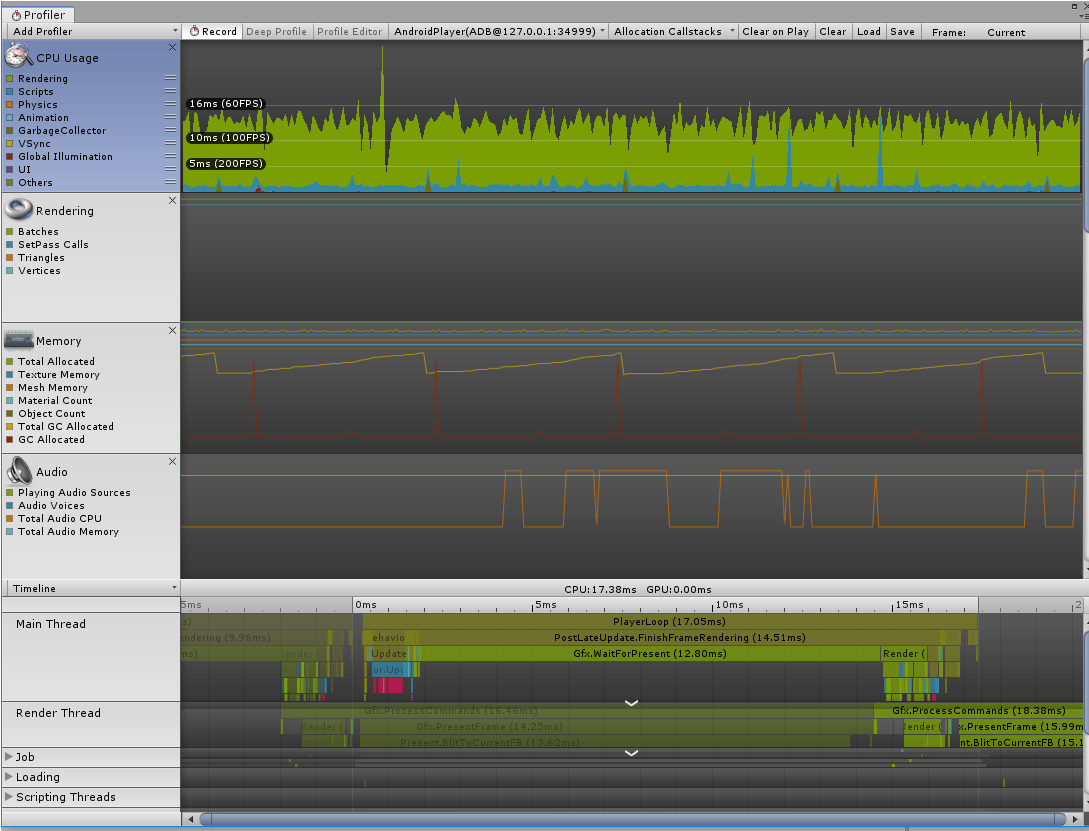
\includegraphics[width=\linewidth]{unityProfiling.png}
    \caption{Unity Profiling Tool}
    \label{fig:unityprofiling}
\end{figure}

Voor deze reden is er een zelfgemaakt script ontworpen om de nodige waarden weg te schrijven naar een csv bestand. Dit script berekent elke second de FPS door het totaal aantal frames van deze second te verminderen met het totaal aantal van de vorige second. Het gereserveerde en alloceerde RAM vraagt het script op aan de UnityEngine.Profiling.Profiler klasse die beide waarden bezit als variabelen. Het script schrijft ook het aantal gameObjects van Unity weg naar de csv, deze waarde kan aantonen wat er juist gebeurt met images eens ze hun tracking verliezen (zie script \ref{code:profilerScript}).

Het script is vast gemaakt aan een leeg gameObject (zonder andere scripts en componenten) om dit te kunnen laten runnen. Het script runt eenmalig zijn Start() functie wanneer het object is geïnitialiseerd en voert dan elke seconde berekening uit.

\codefragment{code/ExperimentProfiler.cs}{Custom Profiler Script}{code:profilerScript}

\section{Applicatie ARCore}

\section{Applicatie Vuforia}

\subsection{Image Database}
De Vuforia image database is aangemaakt via hun developer site. Hierop zijn de 15 afbeeldingen toegevoegd en hebben ze ook elk een score gekregen van 0 tot 5 sterren die aangeeft hoe makkelijk Vuforia de afbeelding kan herkennen (zie figuur \ref{fig:vuforiaDatabase}). Ook is er de mogelijkheid om per afbeelding de features te tonen die Vuforia gebruikt om een afbeelding te herkennen.

\begin{figure}
    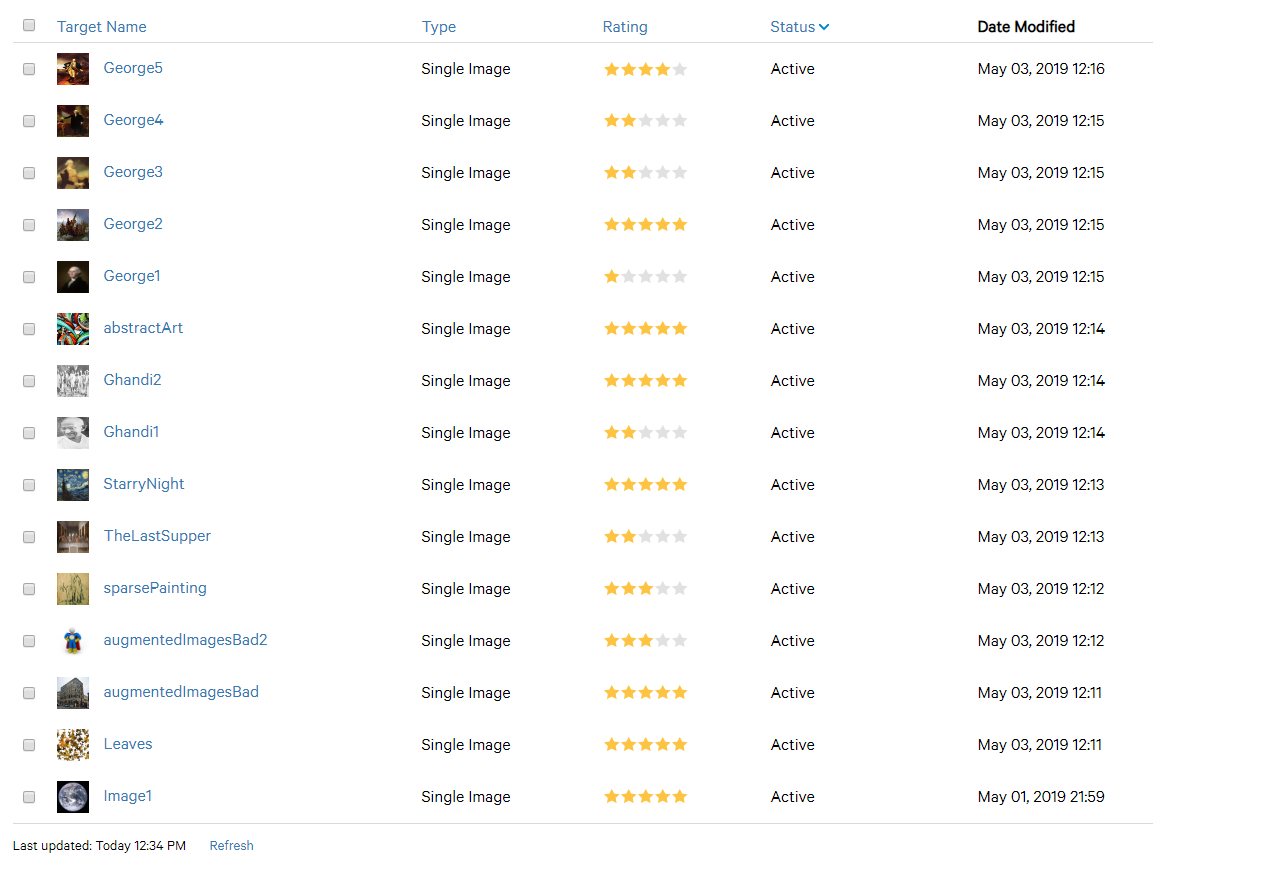
\includegraphics[width=\linewidth]{vuforiaSite.png}
    \caption{Lijst met de 15 images en hun score}
    \label{fig:vuforiaDatabase}
\end{figure}
\subsection{Configuratie}
Om ervoor te zorgen dat Vuforia optimaal gebruik maakt van de platform enablers (in dit geval ARCore) moet eerst de ARCore Unity SDK zich bevinden in het mapje `Assets/Android/Plugins', alleen dan zal Vuforia volledig gebruiken maken van de onderliggende ARCore SDK \autocite{VuforiaARCore}.

Het is ook heel belangrijk dat in de VuforiaConfiguration file bij 'Device Tracker' de optie 'Track Device Pose' is ingeschakeld. Deze optie zorgt ervoor dat Vuforia de image nog eventjes trackt wanneer deze fysiek niet meer zichtbaar is. Ook is hier de optie om te kiezen tussen een 'Positional' of 'Rotational' tracking mode, deze bepaalt het aantal beschikbare \acrlong{dof}. Omdat bij deze applicatie 'Track Device Pose' belangrijk is moet er positional tracking (\acrshort{6dof}) beschikbaar zijn.

%% TODO: Hoe ben je te werk gegaan? Verdeel je onderzoek in grote fasen, en
%% licht in elke fase toe welke stappen je gevolgd hebt. Verantwoord waarom je
%% op deze manier te werk gegaan bent. Je moet kunnen aantonen dat je de best
%% mogelijke manier toegepast hebt om een antwoord te vinden op de
%% onderzoeksvraag.
